\section{Background}\label{sec:background}

The TESS platform builds on previous TS work. In this section we summarize that history (Section \ref{sec:tehistory}) and theoretical context (Section \ref{sec:teecon}).
In the remainder of the paper (\cref{sec:standard_design}), we will show how TESS opens up the closed control architecture of current TS and how it embodies economic theory in its emphasis on price discovery and price-based dispatch to reflect demand and DER value, opportunity costs, and outside options more explicitly in electric systems.

\subsection{Transactive Energy Background}\label{sec:tehistory} 

Transactive energy was originally conceived of as \emph{transactive control} to address the problem of integrating large numbers of small resources optimally into electric power system operations (TE 1.0).
TE 1.0 implemented the ``prices to devices'' concept by pushing a cost-based price signal to devices, observing the response, and changing the price signal iteratively to bring quantity supplied and quantity demanded into equilibrium (a process economists will recognize as Walrasian \emph{tat\^{o}nnement}). This utility-generated price signal tends to be cost-based and supply-focused, reflecting demand only to the extent that devices respond iteratively, with an objective function of achieving a particular system control objective.
This process required large amounts of potentially private information about those resources' supply and demand functions, such as would be required for a formal numerical optimization solution.  This problem has become even more prominent as utilities struggled to integrate a growing variety of behind-the-meter demand response and DERs, including photovoltaics, electrified end-uses that were previously fossil-based, electric vehicles and their chargers, and energy storage into their system operations using conventional utility programs such as energy efficiency and demand-side-management. 

The transactive energy market design developed for the GridWise Olympic Peninsula Testbed Demonstration Project \citep{hammerstrom_2008} moved beyond TE 1.0 (TE 2.0). In a double clock auction buyers and sellers submit bids and offers simultaneously in a specified market time interval. 
The market clears in real-time market and provide a price signal for automated device demand response and dispatch.
The ability to automate device participation in such markets reduces transaction costs, elicits information about relative value and relative cost from agents around the distribution edge via their devices, increases the frequency of participant activity, improves responsiveness, and makes autonomous price-based dispatch feasible. 

Despite the resemblance to a market mechanism, this setup differed from an economic mechanism in several respects. First, the bids did not reflect the actual economic value customers attributed to dispatch, but rather indicated a heuristic technical prioritization, which usually creates circumstances in which devices place bids that are not incentive compatible. However, even though bids did not reflect the true economic value, customers could not deviate from the bid and the assigned dispatch as devices were part of a technical control system. The only option left to customers was to override preferences (e.g., temperature setpoints) and essentially exit the transactive system as a flexible device for the duration of the override. In bidding functions the design task is to express customers' marginal value of dispatch. As a result, customers have no incentive to deviate from their allocation to dispatch and, in addition, market clearing coincides with social welfare optimization. Second, customers were only part of the transactive system, and no other tariff considerations interfered with their market participation (``greenfield''). Customer bidding behavior was therefore guided by the marginal cost of consumption to them (and, likewise, the marginal cost of supply for the utility) \citep{chassin_kiesling_2008}.

Although customers received a lump-sum payment to account for losses they encountered as compared to a fixed retail rate setting, customers consumption decisions were based on their evaluation of the marginal benefit of consumption, and through the market-clearing price they faced the marginal cost of consumption in every market interval. %{\color{red}TKTK, T BIDDING FUNCTION ALGORITHM, SUMMARIZE RESULTS} 
The bidding functions converted comfort objectives, e.g., indoor air temperature, to reservation prices based on the expected price mean and variance. As comfort decreased, the bid price rose above the mean price, and did so more if the price variance was greater. When comfort increased the bid dropped below the mean price, and did so more if the price variance was greater.  The price mean and variance were taken over the past 24 hours, which was very effective at capturing the diurnal nature of comfort and price fluctuations , as shown in  Figure~\ref{fig:Transactive_DA}.

\begin{figure}[t]
\centering
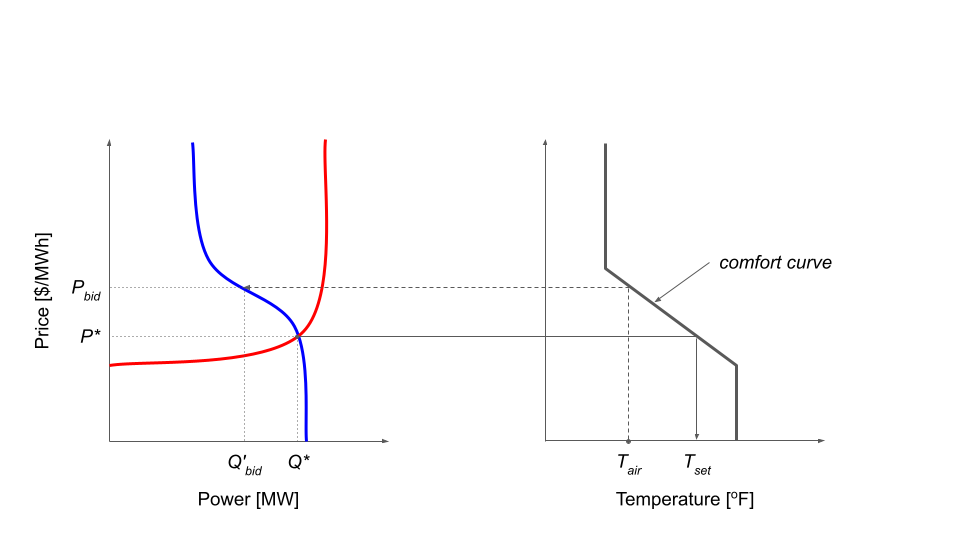
\includegraphics[scale=0.5]{images/TE_DA.png}
\caption{Transactive Double Auction (left) and Thermostat Bidding Strategy (right)}
\label{fig:Transactive_DA}
\end{figure}

This market design with a double auction and automated price-based dispatch forms the foundation for TE 2.0, where the decentralized bid-based and offer-based market changes the paradigm to ``prices from devices'' to establish an informative market-clearing price that is then used for prioritization and dispatch. The TE 2.0 paradigm is more adaptable to unknown and changing conditions and better enables flexibility in the face of uncertainty at varying scales and time frames, and is thus well-suited to the operational challenges associated with increasing DER adoption.

\subsection{Transactive Energy Economic Theory}\label{sec:teecon}

Moving from TE 1.0 to TE 2.0 entails automated active bidding from both demand and supply agents. TESS, our implementation of TE 2.0, employs a synthesis of economic market design and control systems, with an emphasis on demand-side and DER owner/operator bidding \citep{chassin2017thesis}. One of the most important and challenging dimensions of TS design is the design of demand-side and DER bidding. Other TS models tend to fall in one of two categories: basing the device bidding on a cost-based objective, or basing the device bidding function on a technical heuristic or on an aggregate or market demand approximation \citep[Chapter IV]{Arlt2020}. Instead, we propose bidding functions that enable users to communicate their preferences more directly.

The economic foundation of demand-side and DER bidding draws from multiple fields of economic theory \citep{kiesling_2021}. An essential feature of the economics of transactive energy is that people are individually distinct, with subjective preferences over the goods and services they consume. As producers their perceptions of the opportunity costs they face are also subjective. Subjectivism in economic theory reflects the key insight that personal preferences and opportunity costs are private knowledge.

The preferences and opportunity costs of consumers and producers are also not knowable by or accessible to others, so coordination requires some mechanism that gives people incentives to communicate some of that subjective, private knowledge and turn it into information. That mechanism is the price system. A price system operating within a clear set of rules provides a decentralized mechanism for gathering information and learning about these preferences and opportunity costs, even among strangers (or their devices). The market process of mutual learning and decision-making enables prices to emerge that coordinate the actions and plans of all users of the system, incorporating both supply and demand information into that emergent price.

All price systems operate in an institutional framework, a set of rules, and the rules shape the incentives of participants. Effective price systems and market institutions can be challenging, or can fail to exist, due to transaction costs. When transaction costs are high and market transactions are costly to employ for coordination, other methods of organizing economic activity emerge, such as vertical integration. Technological change, most recently digitization and automation, have reduced transaction costs of using the price system relative to these other institutions \citep{kiesling_2016}. The TESS design takes advantage of these transaction cost reductions.

One institutional form for price discovery is auctions. Auctions are useful aspects of market design when the allocation problem is characterized by asymmetric information. In the case of electricity market design, the object for sale has different, subjective value to each potential bidder, a case known as a private value auction model. The double auction (DA), as discussed in Section \ref{sec:tehistory}, treats buyers and sellers symmetrically, enabling them to make simultaneous bids and offers. In a static DA, buyers submit bid schedules and sellers submit offer schedules of price and quantity \citep{friedman1993double}. The centralized auction platform performs a clearinghouse function, arranging all of the buyers’ schedules into a market demand curve and all of the sellers’ schedules into a market supply curve. This process enables a market price to emerge, determining quantity supplied and quantity demanded and clearing the market. Experimental analysis suggests that the DA is a very efficient market design, enabling price discovery even in the presence of fragmented, private knowledge, where each participant knows only her own value/opportunity cost \citep{easley1993theories}.

Another relevant field of economics is mechanism design, a game-theoretic approach to examining situations in which individuals make decisions and interact when they have private knowledge that could affect the decisions they make and the ultimate outcomes. Mechanism design focuses on eliciting truthful revelation of some information about that private knowledge/type. Depending on the environment and the objective function of the principal, different mechanisms can perform better or worse at truthful revelation.

The general structure of mechanism design is to maximize some objective function across all $n$ individuals subject to two constraints: incentive compatibility (IC) and individual rationality or participation (IR). The objective function varies depending on the specific context, but represents profit, surplus, or welfare maximization. The IC constraint ensures that each agent is better off truthfully revealing type in the outcome from the chosen mechanism compared to other alternative outcomes. The IR constraint ensures that each agent is better off participating in the system than not participating. 

Practical mechanisms that can be implemented are hard to identify, and testing such mechanisms is an essential step in overall market design. Experimental economics provides a framework for performing such market design tests, and field deployments are an example of these important tests.

These economic fields and principles inform our overall approach to market design for price discovery, and our design of device bidding functions taking into account opportunity costs and outside options to enable incentive compatible voluntary participation of agents in TESS.



